\documentclass[11pt]{article}
\usepackage{graphicx}
\usepackage{hyperref}
\usepackage{longtable}
\usepackage[margin=.7in]{geometry}


\begin{document}

\title{CSE564 Visualization}
\author{Yinlong Su, \#110461173}
\maketitle

\section*{Row Clean Report}

\setcounter{section}{-1}
\section{Version History}

First built on April 10, 2016.

\section{Row Cleaning}

In the original dataset, there are some illegal rows have wrong data. For example, row 11,865 has wrong data on almost every column (shown in Figure \ref{fig:illegalRow}). It has location information stored in time column, ingredient information stored in product name, etc.
\par
Those illegal rows cause the warning from our csv parser pandas: ``sys:1: DtypeWarning: Columns (0,3,5,27,36) have mixed types. Specify dtype option on import or set low\_memory=False." We remove the rows that has a null value on ``code" column and solve this problem.
\par
The row number reduces from 65,503 to 65,486.

\begin{figure}[!htp]
\centering
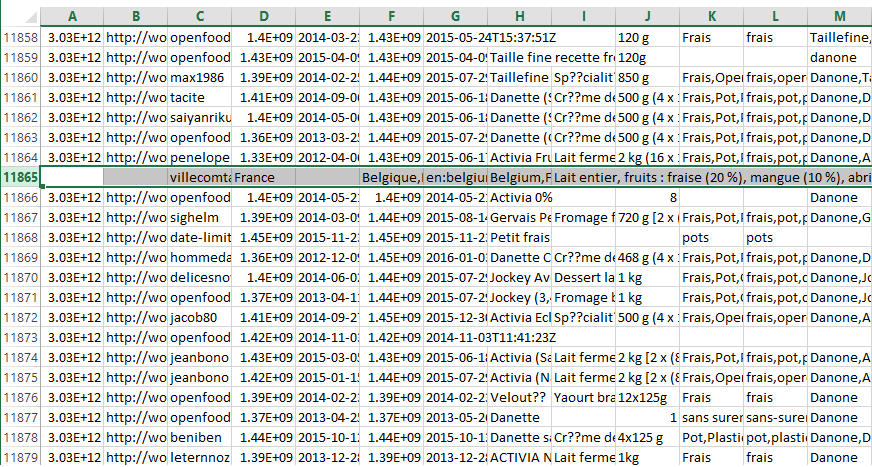
\includegraphics[width=1.0\textwidth]{../vis/illegal.row.png}
\caption{Illegal Row in the dataset}
\label{fig:illegalRow}
\end{figure}

\section{Type Correction}

The ``code" column need to be TextType. Although it contains only number, but the prefix 0s cannot be omitted. And some code numbers are too long to store in an int variable. Indicate the dtype when parsing the csv file.
\begin{verbatim}
    df = pandas.read_csv('row.clean.csv', dtype={'code': str})
\end{verbatim}


\section{Contact Information}
If there is any problem please contact me.
\par
Name: Yinlong Su
\par
SBU ID: 110461173
\par
Email: yinlsu@cs.stonybrook.edu

\end{document}
